\documentclass[tikz,border=6pt]{standalone}
\usepackage[scaled]{helvet}
\renewcommand{\familydefault}{\sfdefault}
\usetikzlibrary{arrows.meta}
\definecolor{ink}{HTML}{12343B}\definecolor{st}{HTML}{BFD9E5}\definecolor{sc}{HTML}{BFE0D3}\definecolor{test}{HTML}{EDC1BB}
\begin{document}
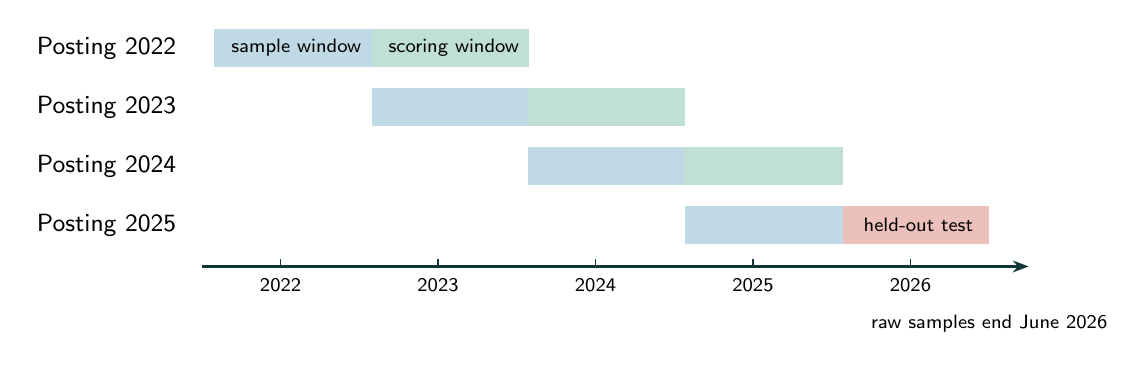
\begin{tikzpicture}[x=20mm,y=7.5mm,font=\small]
% x axis: years from 2021.5; dates are approximate to the month
\foreach \t/\sa/\sb/\ca/\cb/\y/\f in {2022/2021.58/2022.58/2022.58/2023.58/4/sc,2023/2022.58/2023.57/2023.57/2024.57/3/sc,2024/2023.57/2024.57/2024.57/2025.57/2/sc,2025/2024.57/2025.57/2025.57/2026.5/1/test}{
 \node[anchor=east,font=\small] at (2021.5-2021.5-.1,\y) {Posting \t};
 \fill[st] (\sa-2021.5,\y-.32) rectangle (\sb-2021.5,\y+.32);
 \fill[\f] (\ca-2021.5,\y-.32) rectangle (\cb-2021.5,\y+.32);
}
\node at (.6,4) {\scriptsize sample window};
\node at (1.6,4) {\scriptsize scoring window};
\node at (4.55,1) {\scriptsize held-out test};
\draw[-{Stealth[length=2mm]},thick,draw=ink] (0,.3)--(5.25,.3);
\foreach \x/\l in {.5/2022,1.5/2023,2.5/2024,3.5/2025,4.5/2026}{\draw[ink](\x,.3)--(\x,.42);\node[anchor=north,font=\scriptsize] at (\x,.25){\l};}
\node[anchor=north,font=\scriptsize] at (5.0,-.35) {raw samples end June 2026};
\end{tikzpicture}
\end{document}
